\section{Example Usage of the hws Library}
\label{sec:hws_example}

%%% code example
\begin{listing}
    \begin{moderncode}[highlightlines={2, 5-6, 18-19}]{python}
import plssvm
import HardwareSampling as hws
from sklearn.datasets import make_classification as mc

sampler = hws.SystemHardwareSampler()
sampler.start()

sampler.add_event("create")
X, y = mc(n_samples=2**16, n_features=2**11)
svc = plssvm.svm.SVC(C=1.0, tol=1e-8)

sampler.add_event("fit")
svc.fit(X, y)

sampler.add_event("score")
print(f"model accuracy: {svc.score(X, y)}")

sampler.stop()
sampler.dump_yaml("samples.yaml")
    \end{moderncode}
    \caption{%
    A code example showing the simplicity of the hws library. 
    With only five required lines of code, it is possible to gather information from the whole system. 
    Additionally, events can be added to make the final output easier to understand and post-process (lines 8, 12, and 15).
    }
    \label{code:hws_python}
\end{listing}

After the theoretical descriptions of the hws library in the last sections, this section gives a practical example using hws' Python bindings shown in \autoref{code:hws_python} using an \gls{svm} classification task. 
As \gls{svm} implementation, \gls{plssvm} is used, which will be presented in \autoref{sec:blas:plssvm} in more detail. 
The only required lines to collect hardware samples with hws are highlighted. 
In line 5, the used hardware sampler is created. 
The example uses a \code{SystemHardwareSampler}, automatically gathering information from all available and supported hardware platforms in the current system. 
Alternatively, one or more hardware-specific hardware samplers could have been used. 
Since no constructor parameters are provided, all categories are sampled, and the default sampling interval is used. 
In the next line, sampling is started. 
After this, everything is sampled until line 18, where sampling is stopped. 
In line 19, the gathered information is saved to a YAML file. 
Additionally, events can be added to make the final output easier to understand and post-process. 
Although only the Python bindings are shown, the code would look nearly identical when using \cpp since the Python bindings are closely modeled after the \cpp functions and classes. 

%% YAML output example
\begin{listing}
    \begin{moderncode}{yaml}
# the sample category
clock:
  # an exemplary turbostat entry;
  # contains the original turbostat column header name
  average_non_idle_clock_frequency:
    turbostat_name: "Bzy_MHz"
    unit: "MHz"
    values: [3932, 4261, 3525, 3924]
    
  # an exemplary NVML NVIDIA GPU entry
  clock_frequency_max:
    unit: "MHz"
    values: 1440
    \end{moderncode}
    \caption{%
    Exemplary YAML entries. 
    Note that the comments are not output in the YAML file but are only added to this example to facilitate explanation. 
    }
    \label{code:hws_yaml}
\end{listing}

An excerpt from an example YAML file created after the call to the \code{dump_yaml} function is shown in \autoref{code:hws_yaml}. 
The samples are grouped into the different sample categories previously introduced. 
All YAML entries have roughly the same structure: a unit and a value. 
The unit can either be a physical unit like $\si{\mega\hertz}$ in the example, but also, e.g, a simple \texttt{string} in case of the hardware name. 
The second entry is either a single value for fixed samples or a YAML array containing all sampled values. 
In the case of \gls{cpu} entries created via turbostat, the original turbostat header name is also included. 
In addition to the samples, the hardware platform's name, a timestamp when the sampling started, the potential events, the sampling interval, and the time points when the samples were gathered are always reported in the YAML file. 

%%% example plot
\begin{figure}
    \centering
    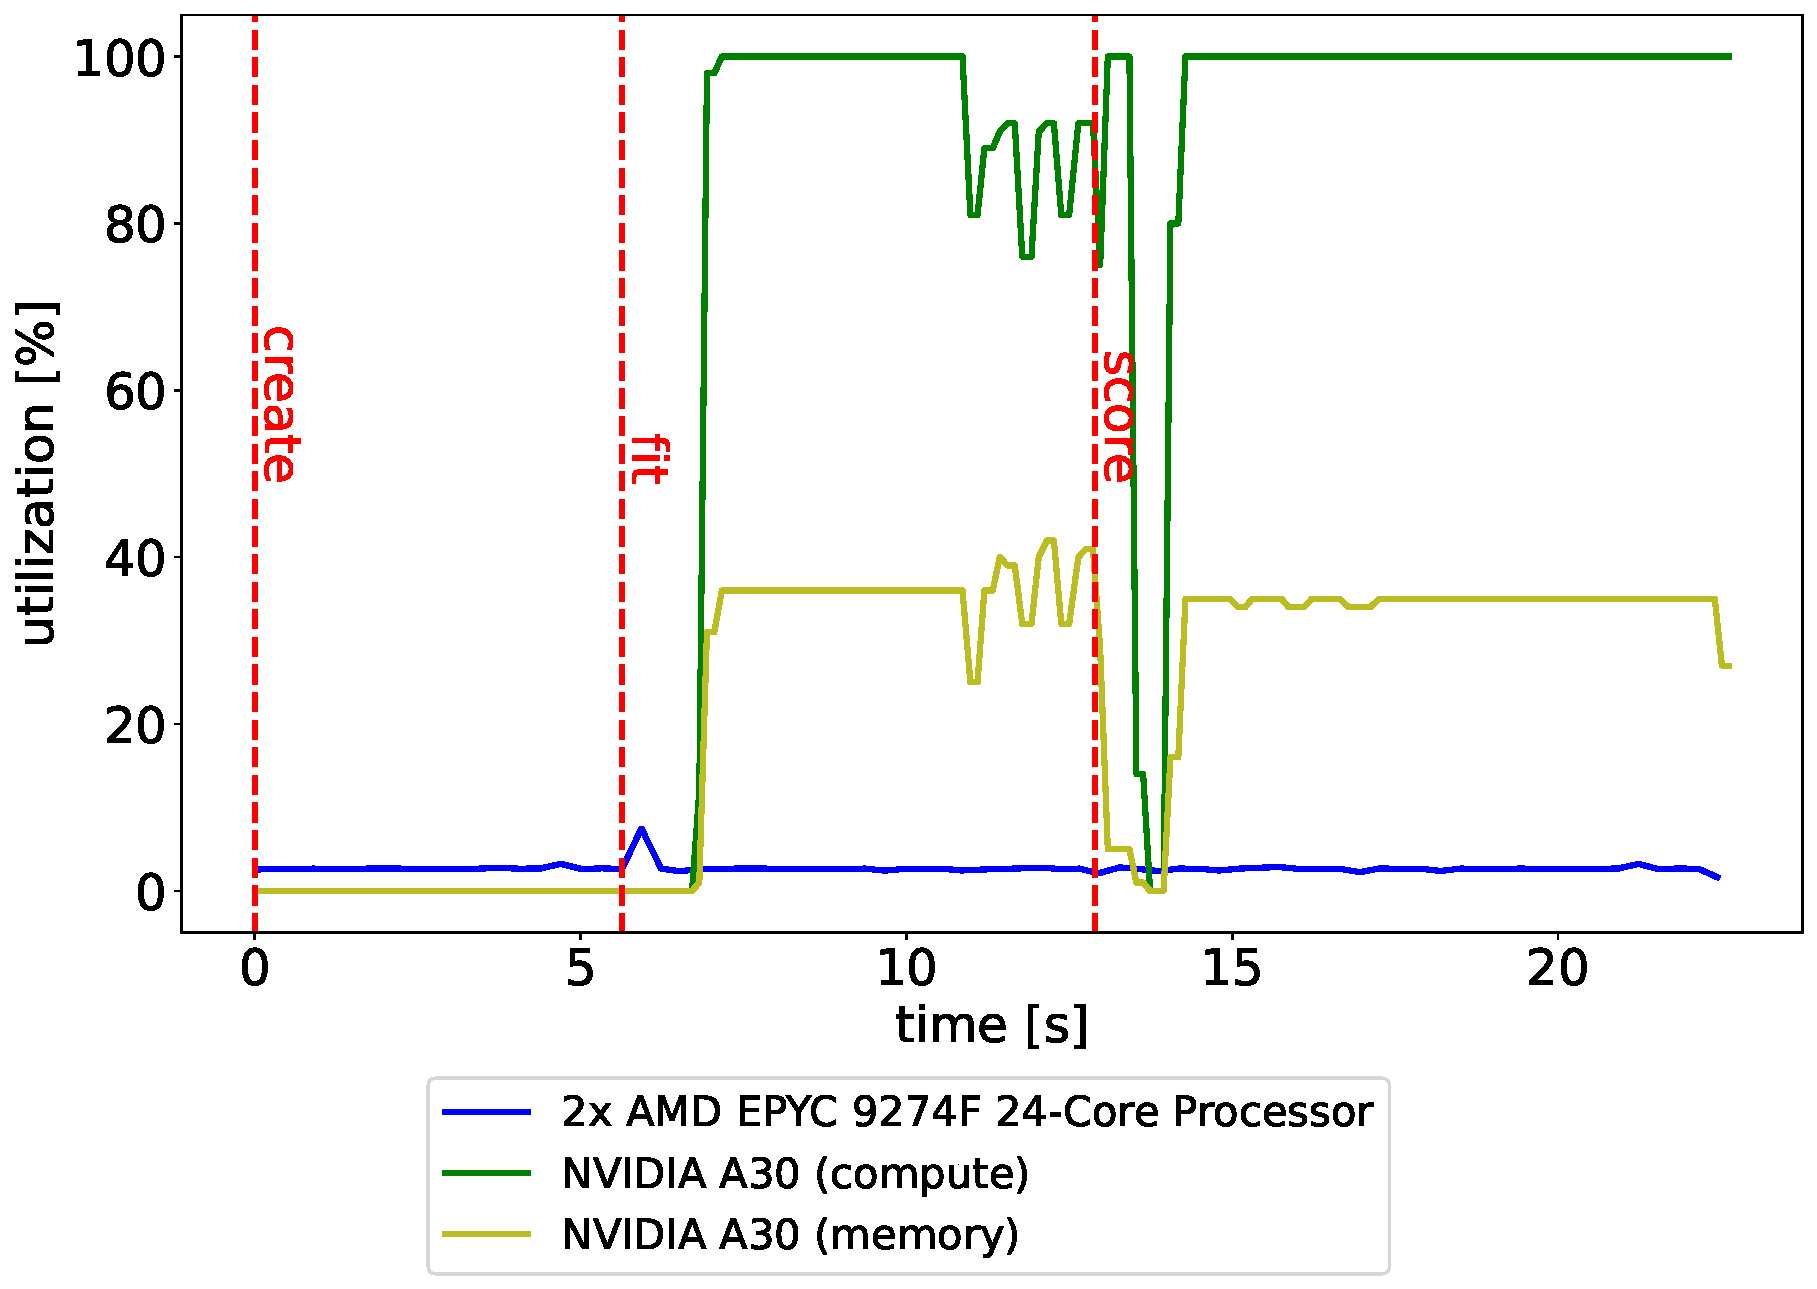
\includegraphics[width=0.85\linewidth]{figures/04_performance_sampling_hws/hws_example_utilization_plot.pdf}
    \caption{%
    The compute and memory utilization of the code shown in \autoref{code:hws_python} executed on a machine with dual-socket \gls{amd} EPYC 9274F \glspl{cpu} and an NVIDIA A30 \gls{gpu}. 
    }
    \label{fig:hws_plot_example}
\end{figure}

This YAML file can be parsed, e.g., using the PyYAML Python library~\cite{simonov_pyyaml_2024} and used to create a plot similar to the one shown in \autoref{fig:hws_plot_example}.
The code from \autoref{code:hws_python} was run on a system with dual-socket \gls{amd} EPYC 9274F \glspl{cpu} and an NVIDIA A30 \gls{gpu}. 
This plot shows the \gls{cpu}s' compute utilization and \gls{gpu}'s compute and memory utilization. 
The three optional events, created in \autoref{code:hws_python} in lines 8, 12, and 15, are added as vertical dashed lines. 
Using the plot annotated with the events, we can easily see the characteristics of the example application. 
The creation of the data set using sklearn's \code{make_classification} function and the initial construction of the SVC classifier are both implemented single-threaded \gls{cpu}-only. 
Therefore, we can see the low \gls{cpu} and no \gls{gpu} utilization. 
Next, the SVC classifier is fitted on the data set. 
At first, setup tasks on the \gls{cpu} must be performed, followed by assembling a kernel matrix on the \gls{gpu}. 
Here, the compute utilization of the \gls{gpu} is $\SI{100}{\percent}$. 
After the kernel assembly, a \gls{cg} algorithm is used to solve a system of linear equations. 
However, only parts of this \gls{cg} are implemented on the \gls{gpu} shown by the worse compute utilization. 
We can also see the different \gls{cg} iterations. 
The SVC fitting is followed by scoring the same data set. 
Again, at the beginning, we can see a setup phase on the \gls{cpu} followed by the \gls{gpu} kernel also achieving $\SI{100}{\percent}$ compute utilization. 
A similar trend can be seen in the memory utilization, although it is at most only $\SI{36}{\percent}$.


%%% overhead for the example
\begin{figure}
    \centering
    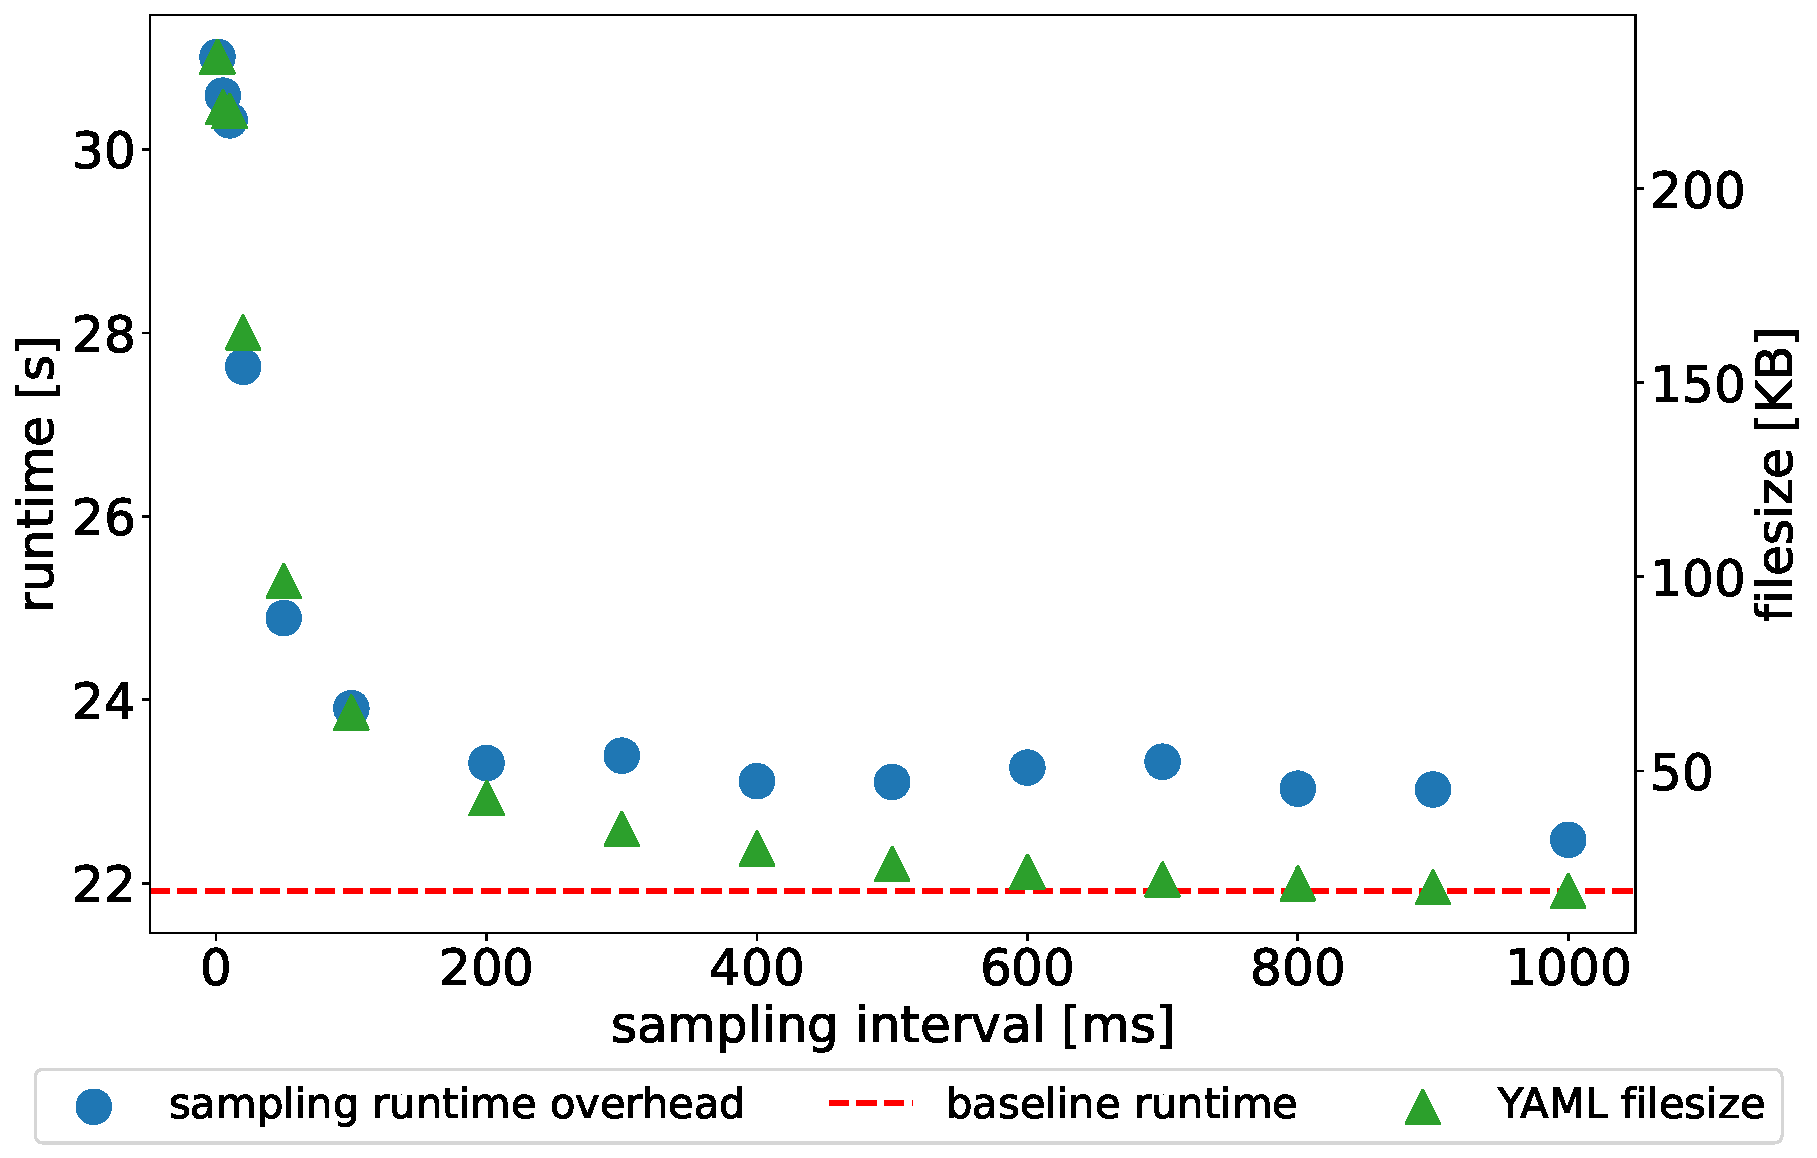
\includegraphics[width=0.8\linewidth]{figures/04_performance_sampling_hws/hws_sampling_interval_overhead.pdf}
    \caption{%
    The overhead, runtime and YAML file size, when using the hws library depending on the sampling interval used. 
    The red dashed line at the bottom is the baseline runtime without the hws library enabled. 
    As a code example, the code from \autoref{code:hws_python} was used. 
    }
    \label{fig:hws_overhead}
\end{figure}

Since sampling the hardware information itself incurs some overhead, this may impact the performance of the actual user application. 
\autoref{fig:hws_overhead} shows the runtime overhead of \autoref{code:hws_python} when using different sampling intervals on the same machine used for \autoref{fig:hws_plot_example}. 
For all tested sampling intervals, an overhead compared to the baseline runtime of $\SI{21.91}{\second}$ without hardware sampling can be seen. 
Using a sampling interval of only $\SI{1}{\second}$, the overhead is the lowest with only $\SI{2.55}{\percent}$. 
This overhead stays relatively constant until a sampling interval of $\SI{200}{\milli\second}$ and further increases for smaller sampling intervals. 
In this example, the default sampling interval of $\SI{100}{\milli\second}$ has an overhead of $\SI{9.10}{\percent}$ with a runtime of $\SI{23.91}{\second}$ while the highest overhead of $\SI{41.51}{\percent}$ is reached with the lowest supported sampling interval of $\SI{1}{\milli\second}$. 
This overhead of over $\SI{40}{\percent}$ is quite high. 
However, the hws library is meant to gather a broad overview of the hardware characteristics when executing a code. 
It is not meant to be used to gather extremely fine-grained information. 
Therefore, even though it is theoretically supported, it is not advisable to use a very small sampling interval. 
With a sampling interval in the range of a few hundred milliseconds, we can still get meaningful information with only a rather small runtime overhead. 

\autoref{fig:hws_overhead} additionally shows the sizes of the resulting YAML files for each sampling interval. 
It should not be surprising that the file sizes increase with smaller sampling intervals since more data is gathered. 
In the example, the sampling interval of $\SI{1}{\milli\second}$ results in a YAML file of $\SI{234}{\kilo\byte}$ while the same YAML file has only the a size of $\SI{19}{\kilo\byte}$ with a sampling interval of $\SI{1}{\second}$. 
Note that the YAML file is not expected to get smaller if we increase the sampling interval further since the file size converges to the size necessary to store all fixed samples that are always gathered, irrespective of the used sampling interval. 
